\section{Illustrative scenarios}
\label{sec:study}

In this section we present two illustrative scenarios, usingq census data from
the United States~\citep{nhgis} and
Canada\footnote{\url{http://datacentre.chass.utoronto.ca/census/}}, tabulated by
CTs,  from 1970 to 2010. 

The prototype interface allows access to 41 regions, 29
in the US and 12 in Canada. New York City was split into its boroughs to avoid
memory crashes on the client browser due to the high number of CTs.  We used
five aspects for the USA: Education level, Family income, Marital status,
Occupation, and Race; and seven for Canada: Age, Education level, Home language,
Household Income, Marital status, Occupation, Place of birth, and Religion. 

While our method does not require geographic harmonisation, it requires matching
the variables over time. The supplementary material contains the details of
which census columns were used for each aspect. Income is slightly inaccurate,
even though we did correct for the official inflation. We grouped the original
ranges into three larger ranges, but they do not match precisely.

\revision{Accidentaly, the US data for 2010 is actually not from the decennial
census, but from the ACS 2006-2010. Further, the regions selected do not
correspond to any pre-defined regions (metros, cities, census areas), but to
arbitrary regions defined around a location of interest. We selected a minimal
set of aspects for each country, and they are not similar to each other, out of
convenience, since the variable matching was a manual process. These caveats
would likely compromise any serious attempt on a comprehensive demographic
study, but this is not the objective of this experiment. These results are meant
to demonstrate the utility of the interface for understanding the evolutionary
dynamics of urban neighbourhoods. They also show the face validity of the
results generated by our novel network-based approach. Indeed, our results were
perfectly aligned with several other studies, despite these methodological
missteps, which could arguably be an indicator of its robustness.}

\subsection{Chicago}
Our first scenario examines Chicago, focusing on a region loosely following the
City's administrative borders. Its demographic composition is well explored in
the literature, with reports of racial divide and
gentrification~\citep{Delmelle2016,Delmelle2017,Hwang2014}, so we expect our
results to contain stable regions where the Race aspect is relevant, and some
degree of population change, with increasing income and education levels. 


The initial state of the prototype is illustrated in Figure~\ref{fig:ui}. The
first step is to identify the compositions of each cluster from the boxplots, so
orange is associated with majority of White population, green with majority
Black, and purple with higher proportion of four years of college or more (high
education level). The expanded version of the boxplots for the purple cluster
shows a higher income level and majority of occupations in administrative jobs,
therefore the purple cluster identifies gentrified regions.


The trajectories plot illustrates the process of gentrification, also
illustrated in Figure~\ref{fig:chiWorkflow}, progressively absorbing regions
from the orange cluster (White). This corroborates results from the literature
reporting that Black neighbourhoods are less likely to
gentrify~\citep{Hwang2014}. Moreover, this process appears to be unidirectional,
as indicated by the limited number of trajectories leaving the purple stream.
Next, we select the region that is gentrified in 2010, by clicking on the
corresponding rectangle in the trajectories plot, updating the information on
the maps and the details portion of the interface.

The corresponding regions are highlighted in the maps, where the spatial pattern
is clear, corresponding exactly to previous findings in the literature based
upon harmonisation~\citep{Hwang2014}. Further, we can also identify the regions
that gentrified earlier on the small maps that depict the involved regions over
time. Since the most relevant aspect is Education, specifically "Four or more
years of college", we can expand the details of this aspect, as illustrated in
the rightmost portion of Figure~\ref{fig:chiWorkflow}, which is increasing for
the whole city (grey band), but faster and to a higher level in this region
(black band).



\begin{figure*}
    \centering
 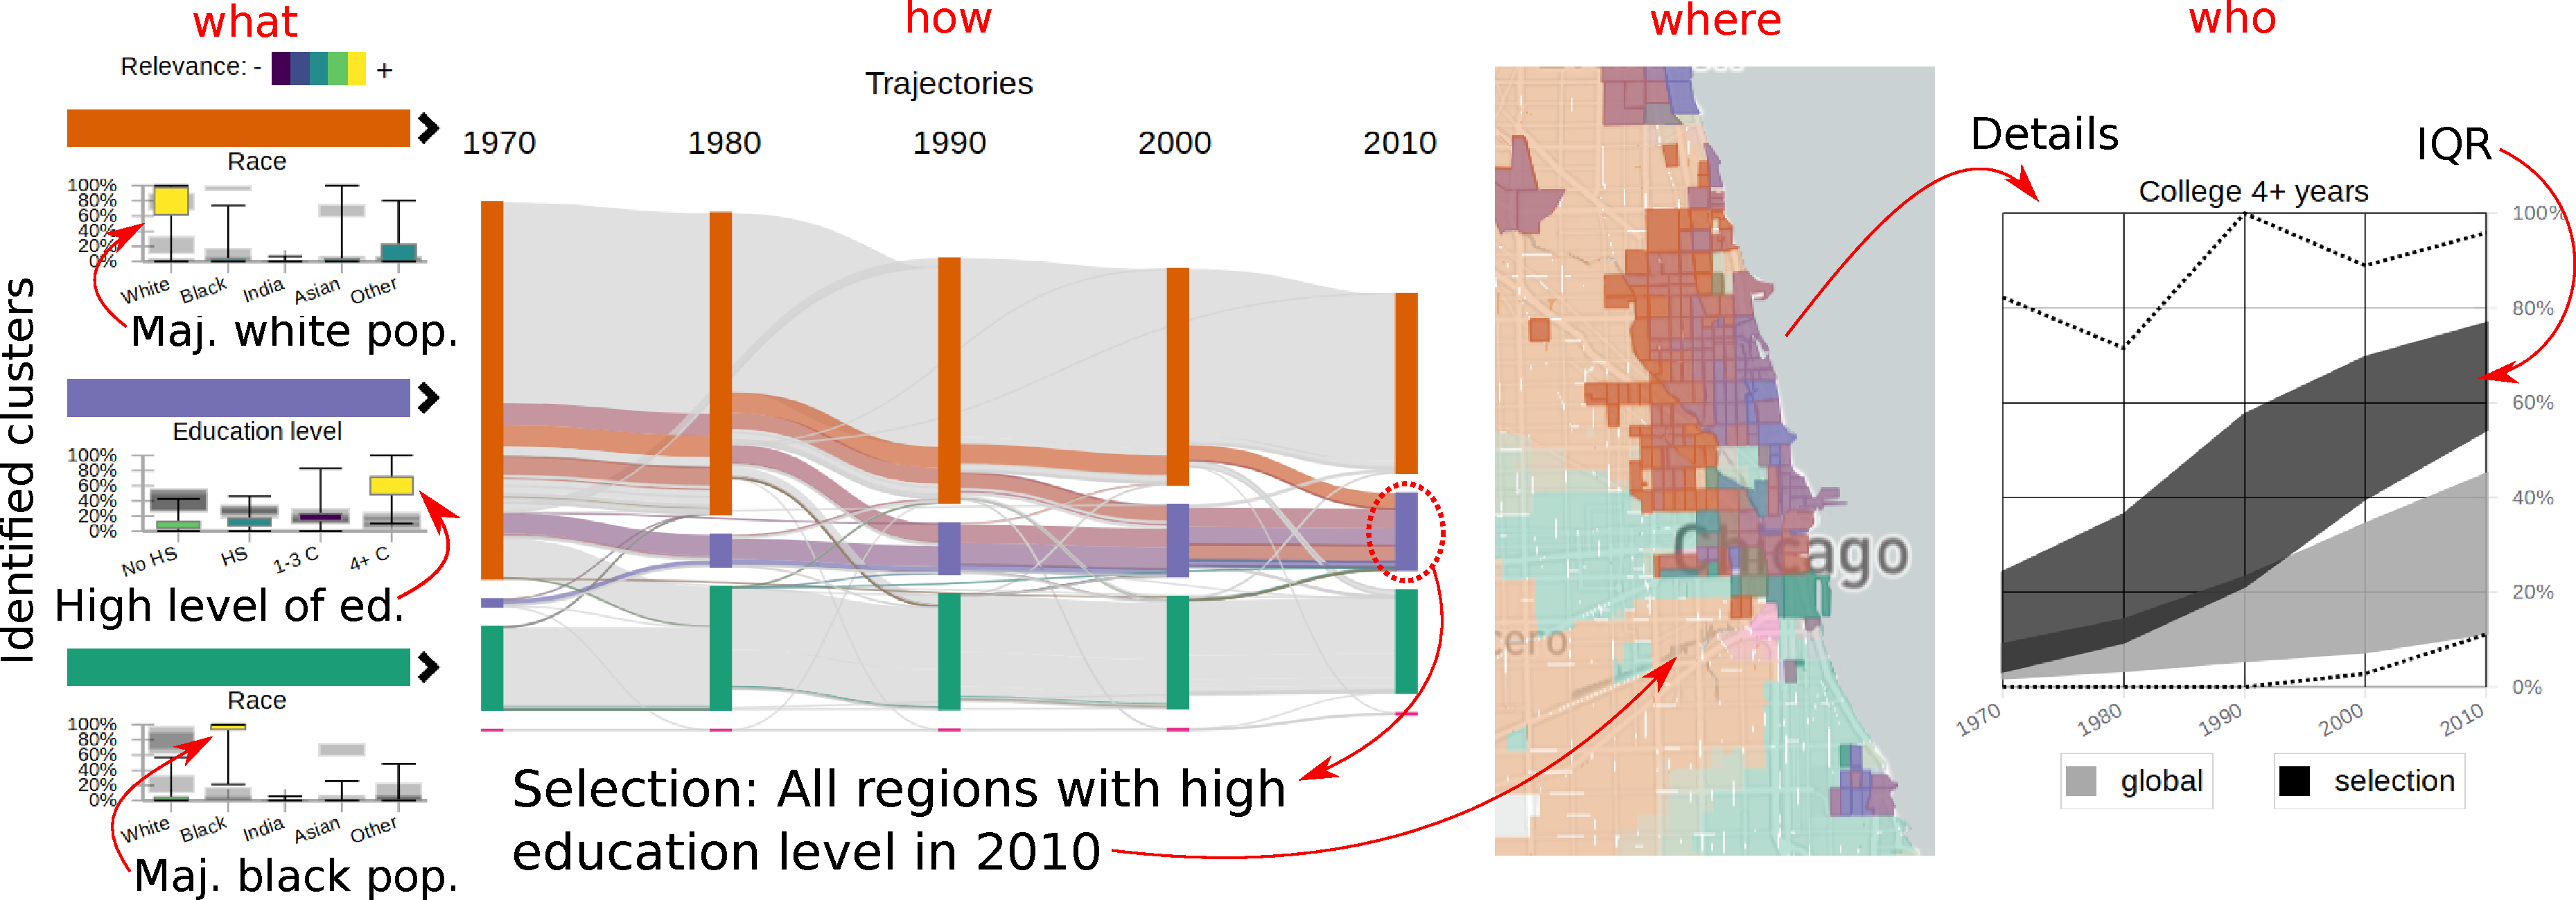
\includegraphics[width=0.9\linewidth]{newTeaser.pdf}
 \caption{Workflow to discover gentrification in Chicago: the purple cluster
 corresponds to high education / income. Its population is increasing over time,
 absorbing from the majority White cluster (orange). By selecting the purple
 cluster in 2010, the region is highlighted in the maps. The proportion of
 people with 4+ years of college is increasing in the whole city (grey IQRs),
 but significantly more in this region (black).\label{fig:chiWorkflow}}
\end{figure*}



\subsection{Toronto}

We consider a region that corresponds approximately to the administrative border
of the current city of Toronto, using all seven available aspects with equal
weights. While Chicago was fairly stable, Toronto is known to be a more dynamic
and diverse city, with significant and increasing immigrant
population~\citep{hulchanski2007three,Fong2011}, especially
Asian~\citep{Fong2003}. Toronto is also known for a stable and well defined
Jewish community~\citep{Harold2018, Fong2011}. Therefore, we expect a
combination of stable and dynamic regions on the results, with Place of Birth,
Home Language, and Religion identified as relevant aspects. The results are
summarised in Figure~\ref{fig:to}, considering eight clusters.

\begin{figure}
    \centering 
    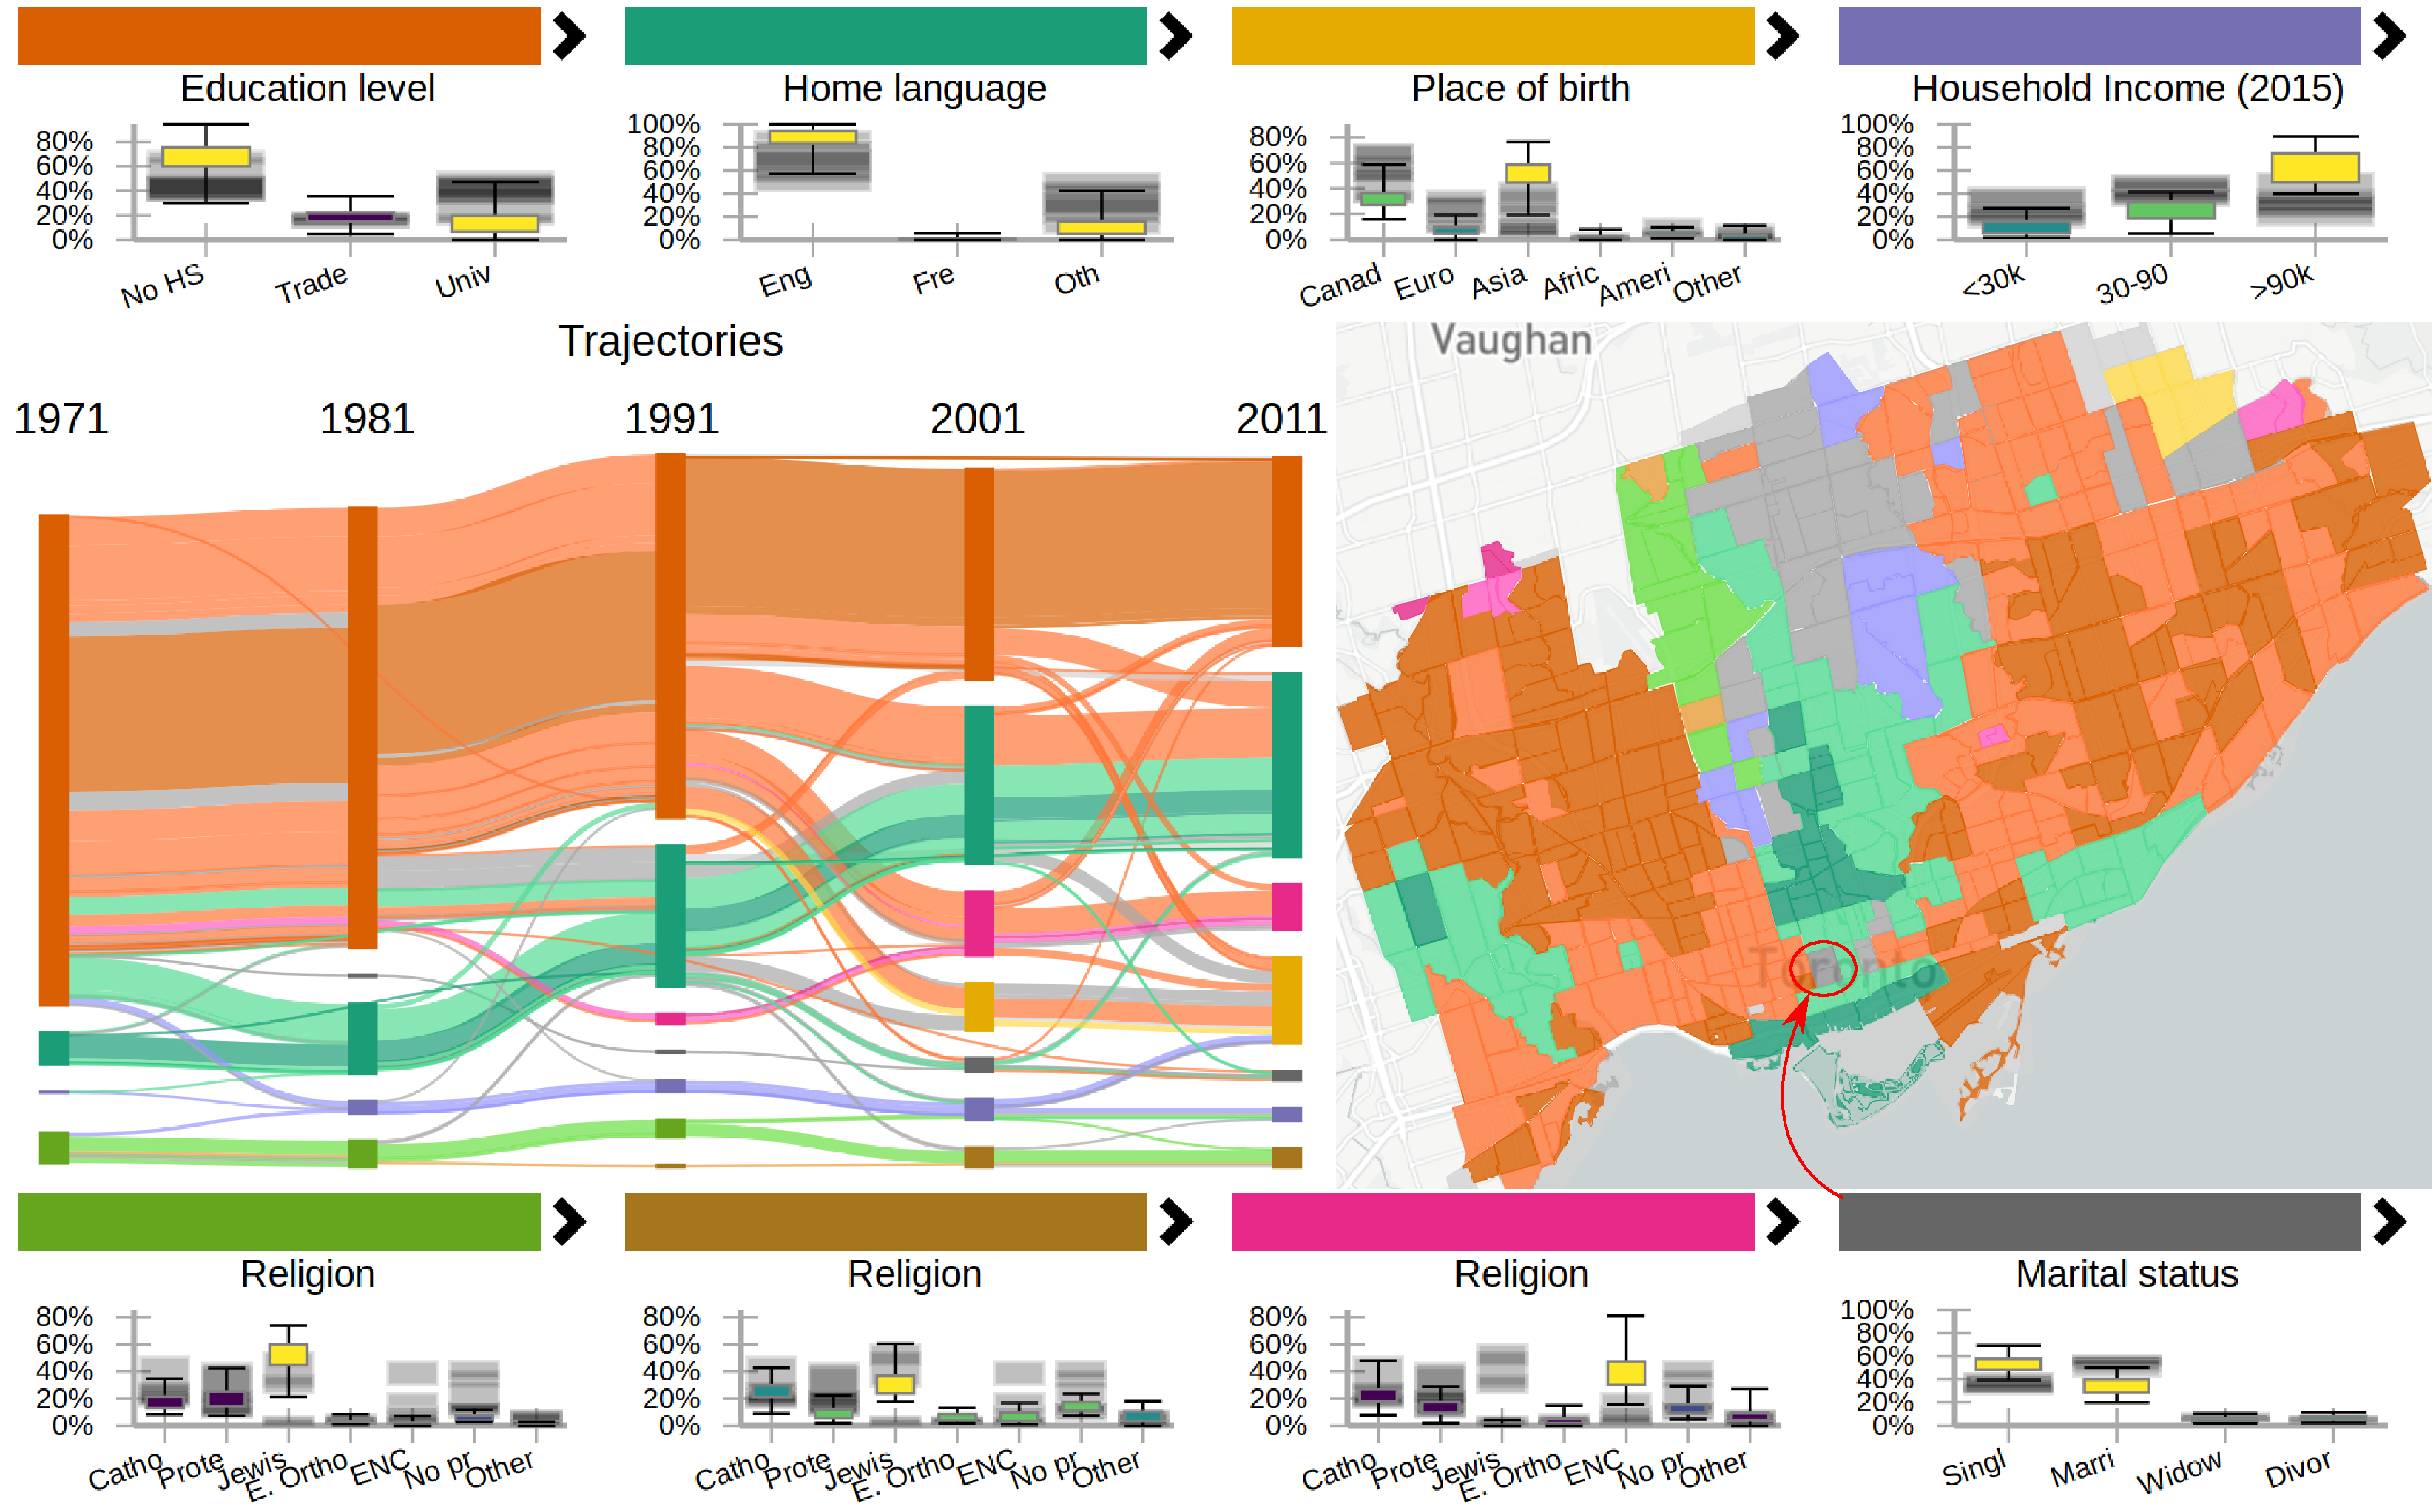
\includegraphics[width=0.85\linewidth]{to.pdf}
    \caption{Clustering results for Toronto, with eight clusters, including
    clusters representing Jewish population, high and low income, low education,
    and Asian immigration.\label{fig:to}}
\end{figure}

The population with low percentage of University degrees is represented in
orange, mostly anglophone population in green, Asian immigrants in yellow, high
percentage of income in the highest bracket in purple, high percentage of Jewish
people in light green and brown, high percentage of Eastern Non-Christian
religion in pink, and high concentration of single people in dark grey. From the
trajectories plot, we can see that Toronto is more dynamic than Chicago, with
one cluster constantly shrinking. In the 1970s, the city was divided into four
clusters: low number of university degrees, Jewish population, majority
anglophones, and high income. Interestingly, the more recent clusters that
absorbed regions from the orange cluster have similar education profiles and are
differentiated by other aspects. In this sense, the city is growing diverse,
changing from a common low education profile to a higher level of education with
more diversity in religion (pink) and immigration (yellow).


Indeed, the growing Asian population is visible starting in the 1980s and
building thereafter, leading to the yellow and pink clusters. While both include
a high percentage of people born in Asia, the pink is more defined by religion,
with low percentage of university degrees, and contains the lowest percentage of
people in the highest income bracket for these clusters; the yellow is less
defined by religion, and has higher education and income, geographically
corresponding to the Markham region, know for its Chinese population. A similar
division also happens for the two Jewish clusters, where the light green cluster
has lower education and income levels than the brown cluster. The purple cluster
of high income is somewhat stable. Until 2011 the cluster included the Bridle
Path neighbourhood, known for its wealthy population. In 2011 it was classified
into the yellow cluster of Asian immigration, since about 40\% of the population
for this CT were then born in Asia. The income distribution did not change, with
85\% of the population with an income of 90k CAD or more.


The most significant indicator of Toronto's dynamism is the presence of grey
regions on the map. These represent regions associated to three or more clusters
over this five census period. Using the 'Add' mode for the trajectory selection,
we select their trajectories, and a subset of the details is illustrated in
Figure~\ref{fig:toVol}. These regions account for about 5\% of Toronto's
population. The whole region was classified into the orange cluster in 1971 (low
level of university degrees). By 1991, most of the region was classified into
the green cluster, representing anglophone population, mostly Canadian born,
with a higher level of education. As the corresponding plot indicates, this
trend in increasing education is city-wide, but this region has people with
better education than most.

\begin{figure}
    \centering 
    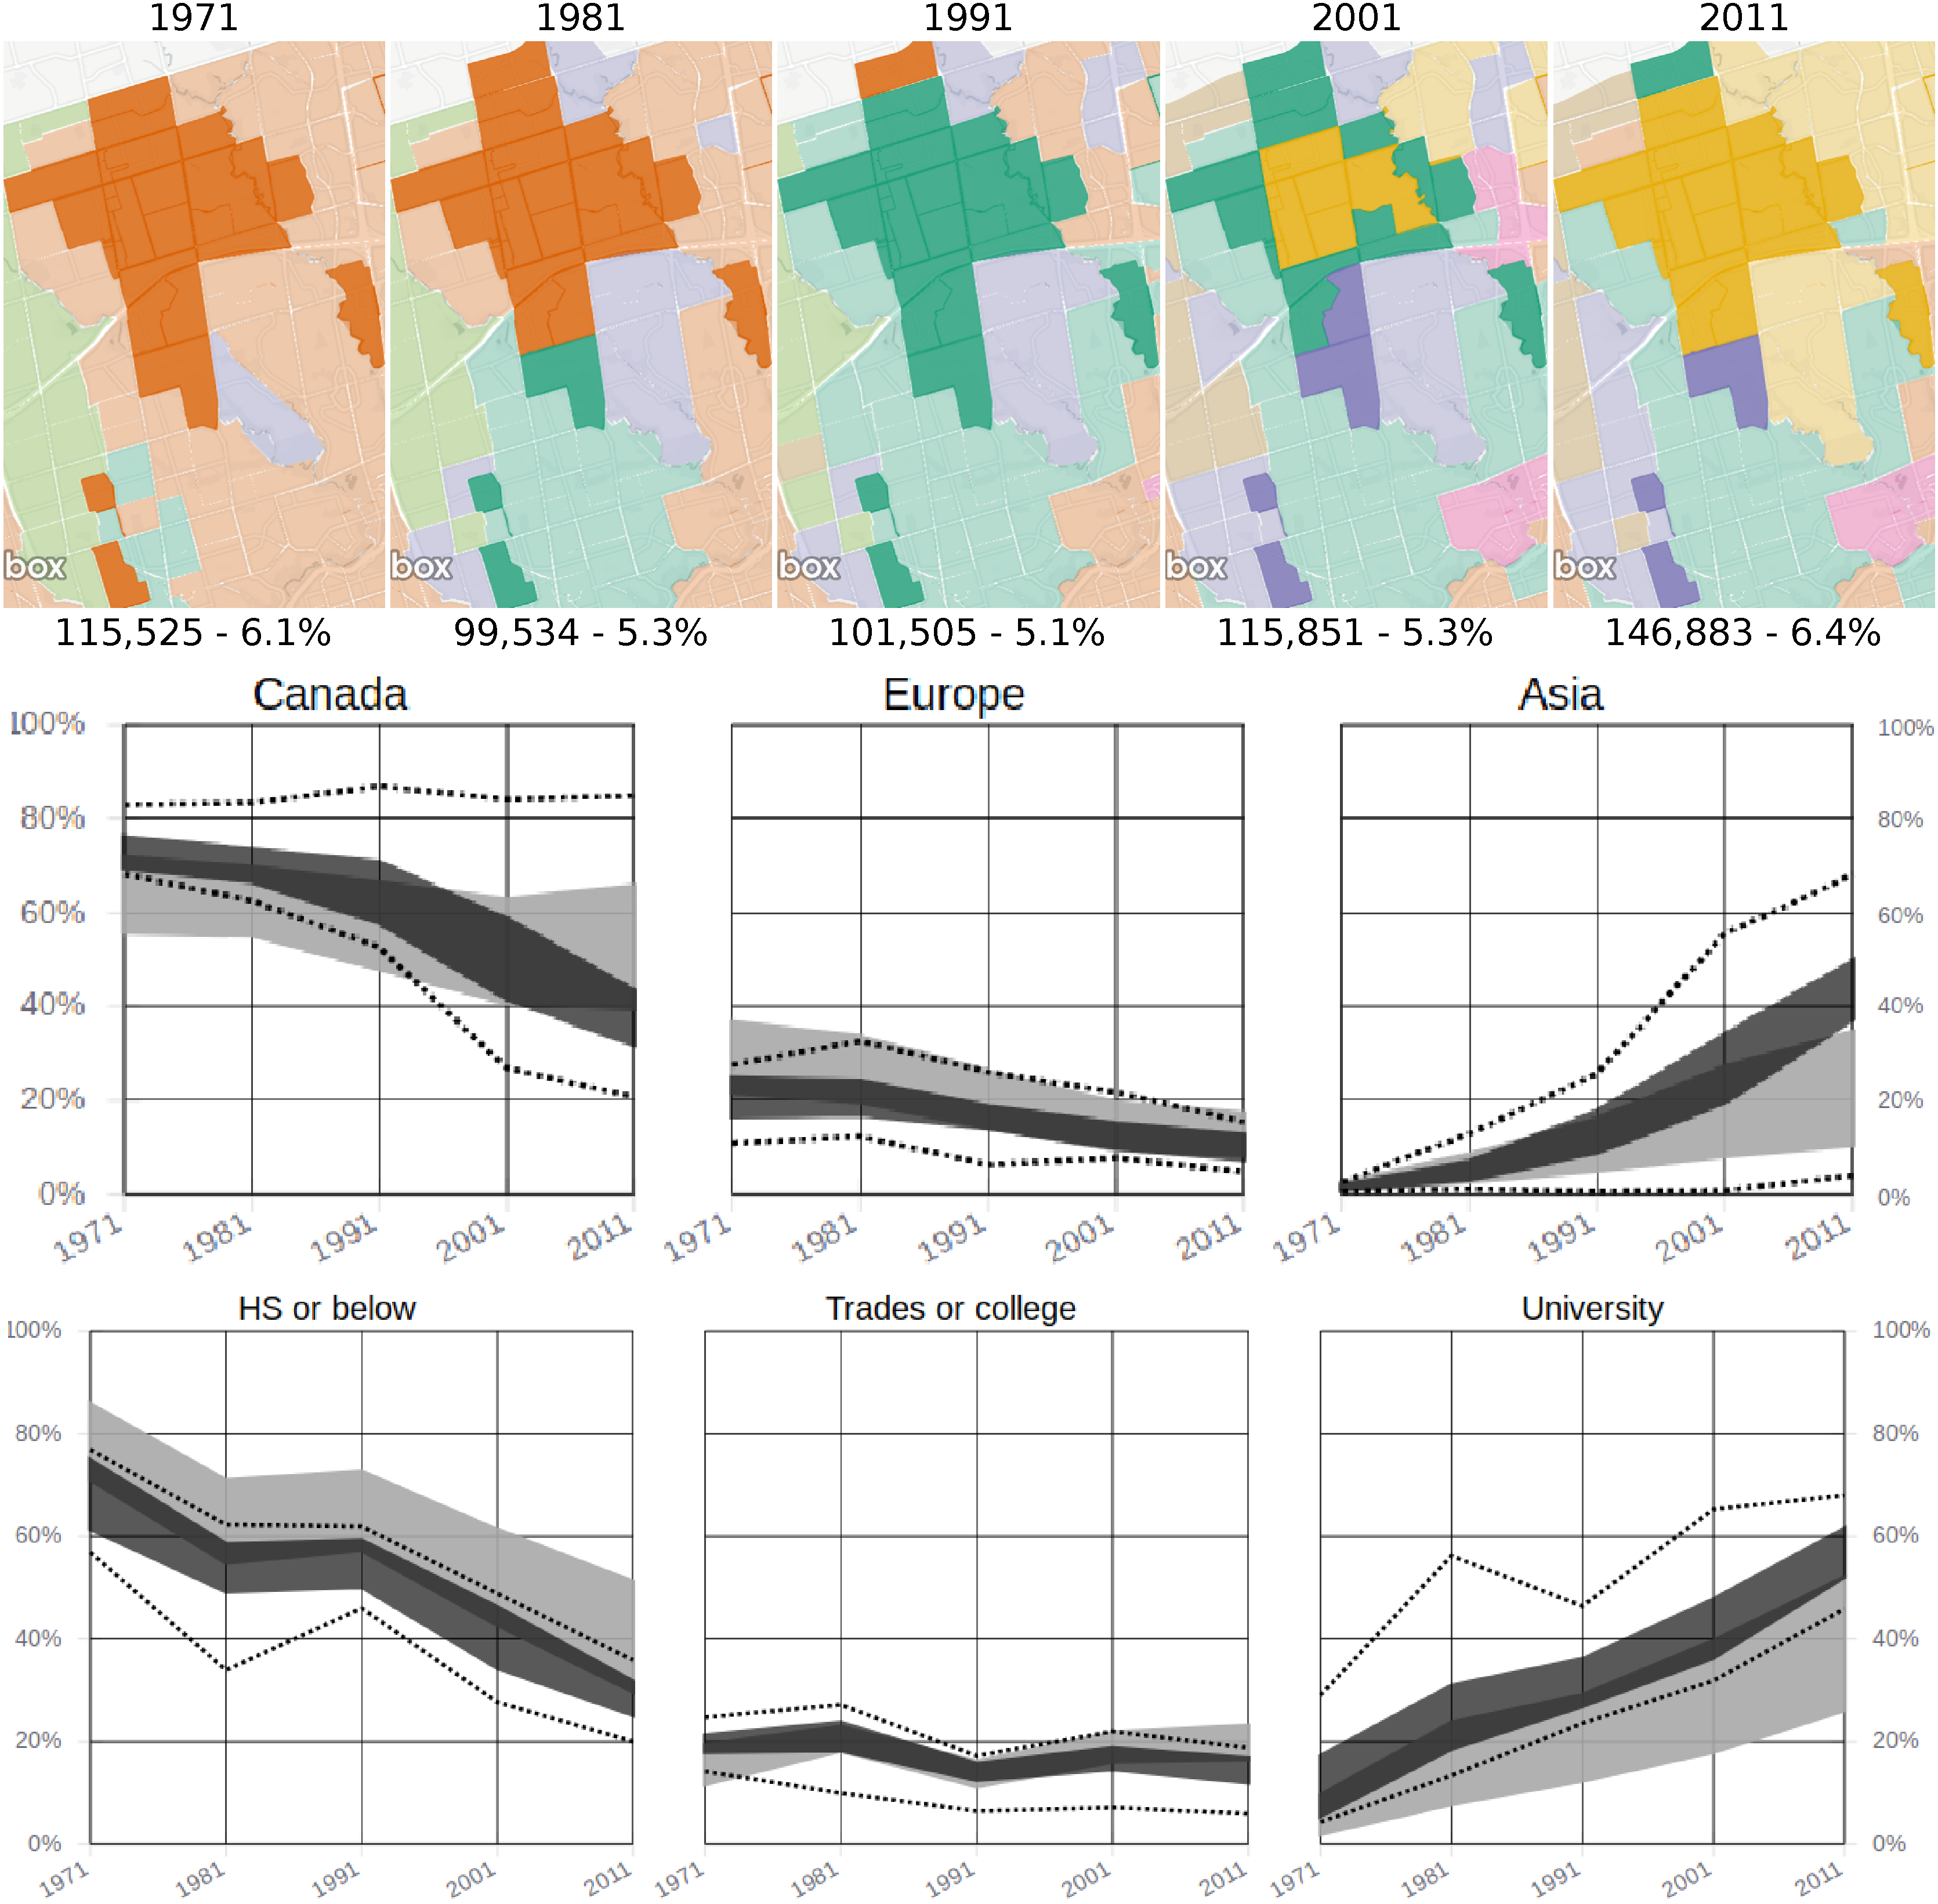
\includegraphics[width=0.75\linewidth]{toVol.pdf}
    \caption{Details for some regions of Toronto that were classified into 3 or
         more clusters over time.\label{fig:toVol}}
\end{figure}

In 2001, the purple cluster of high income annexes neighbouring parts of the
volatile region, and the Asian born population increases sharply, as illustrated
by the appearance of the yellow cluster.  This cluster indicates well educated,
higher income, and about 30\%-50\% Asian born population. By 2011, the yellow
cluster increased considerably, annexing parts of the high income purple
cluster, including the neighbouring Bridle Path area.

The geographical borders of the clusters obtained using our method are similar
to the regions presented by previous studies considering
Toronto~\citep{hulchanski2007three}. However, our interface provides a deeper insight
into their demographic composition, since we consider more data than solely
Average Income, which appears to be a good proxy variable nonetheless. This
scenario showcases the ability of our method and interface to capture and
understand the sources of urban volatility.

% \subsection{Los Angeles}

% We selected for this scenario a region around the metropolitan area of Los
% Angeles (LA), following urban density. While Chicago and Toronto demonstrated
% the abilities of our method to examine stable and dynamic cities, LA is considerably
% larger, both in population and area. Since our method identifies only the eight
% most distinct groups, we expect that some groups will not be identified,
% especially if their characterisation is similar to another groups. Further, our
% system does not include the census variables related to Hispanic heritage, which
% were only included in the newer censuses. However, from the literature, we
% expect to see some clusters where Race is an important aspect, including White,
% Black, and Asian~\citep{Reibel2003}.




% The summary of the results using all aspects with equal weights and eight
% clusters is illustrated in Figure~\ref{fig:la}. The full statistical description
% of the clusters is illustrated in Figure~\ref{fig:laAll}, where the most
% relevant aspect of each cluster is highlighted. From the trajectories plot, we
% can see that there is a large but shrinking cluster, depicted in green, one
% increasing cluster in purple, an almost constant orange cluster, a smaller but
% increasing pink cluster, and three other small clusters. The corresponding map
% illustrates where these clusters are located, and that they are somewhat
% geographically stable, with some movement between the green, orange, and purple
% clusters.

% \begin{figure}
%     \centering 
%     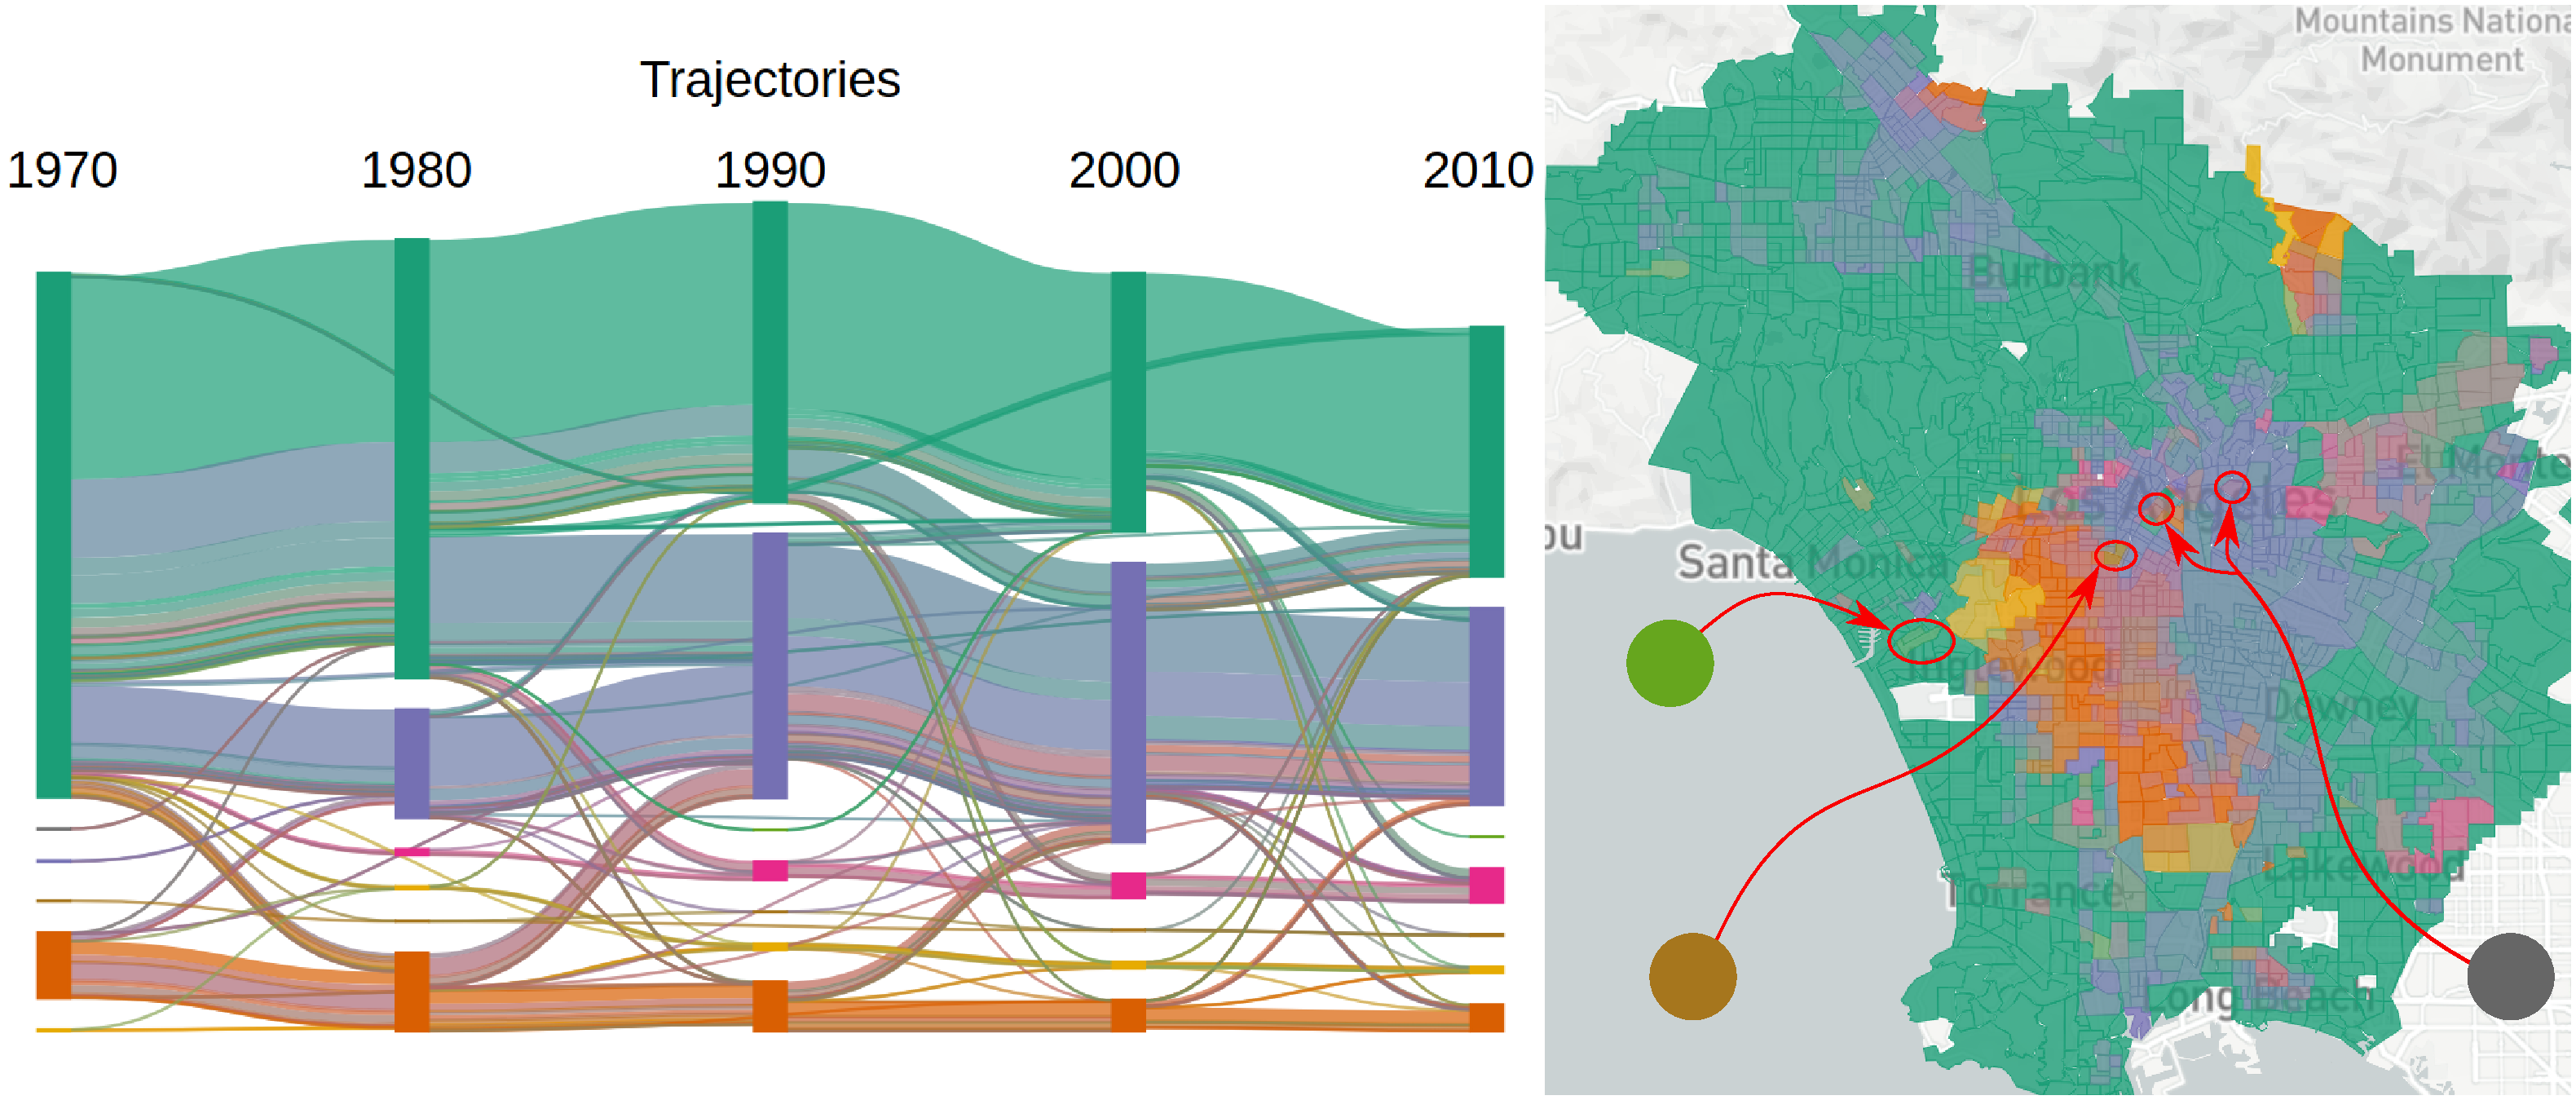
\includegraphics[width=0.975\linewidth]{LA.pdf}
%     \caption{Result for Los Angeles with 8 clusters, including three small and
%         ephemeral clusters. Cluster characterisation is displayed
%         in Figure~\ref{fig:laAll}.\label{fig:la}}
% \end{figure}

% From Figure~\ref{fig:laAll}, we can see that the green cluster is characterised
% by a high percentage of White population, low percentage of population in the
% lowest income bracket, mostly administrative occupations, and about 30\% of the
% population with four or more years of college. The orange cluster is
% characterised by a high percentage of Black population, with few people in the
% highest range of income and education. The purple cluster corresponds to a high
% concentration of "Other" in race, which includes Hispanic for this dataset, high
% concentration of Labourers, and low education and income. The pink cluster
% contains a high percentage of Asian population and about 30\% of the population
% with four or more years of college. The light green cluster contains very few
% people in the lower income bracket, mostly White population, with the highest
% percentage of population with four or more years of college, working
% administrative jobs, and a high concentration of singles. The yellow cluster
% represents Black population, with higher level of education and income, mostly
% working administrative jobs. The brown cluster represent a majority of single
% population, working administrative jobs with mostly low income. The dark grey
% cluster is characterised by all its population in the lowest income bracket, low
% education level, with a majority of White population. Since the extremes in the
% boxplots of the grey cluster are not significantly different, we can also
% surmise that this cluster is either small or homogeneous.

% \begin{figure*}
%     \centering 
%     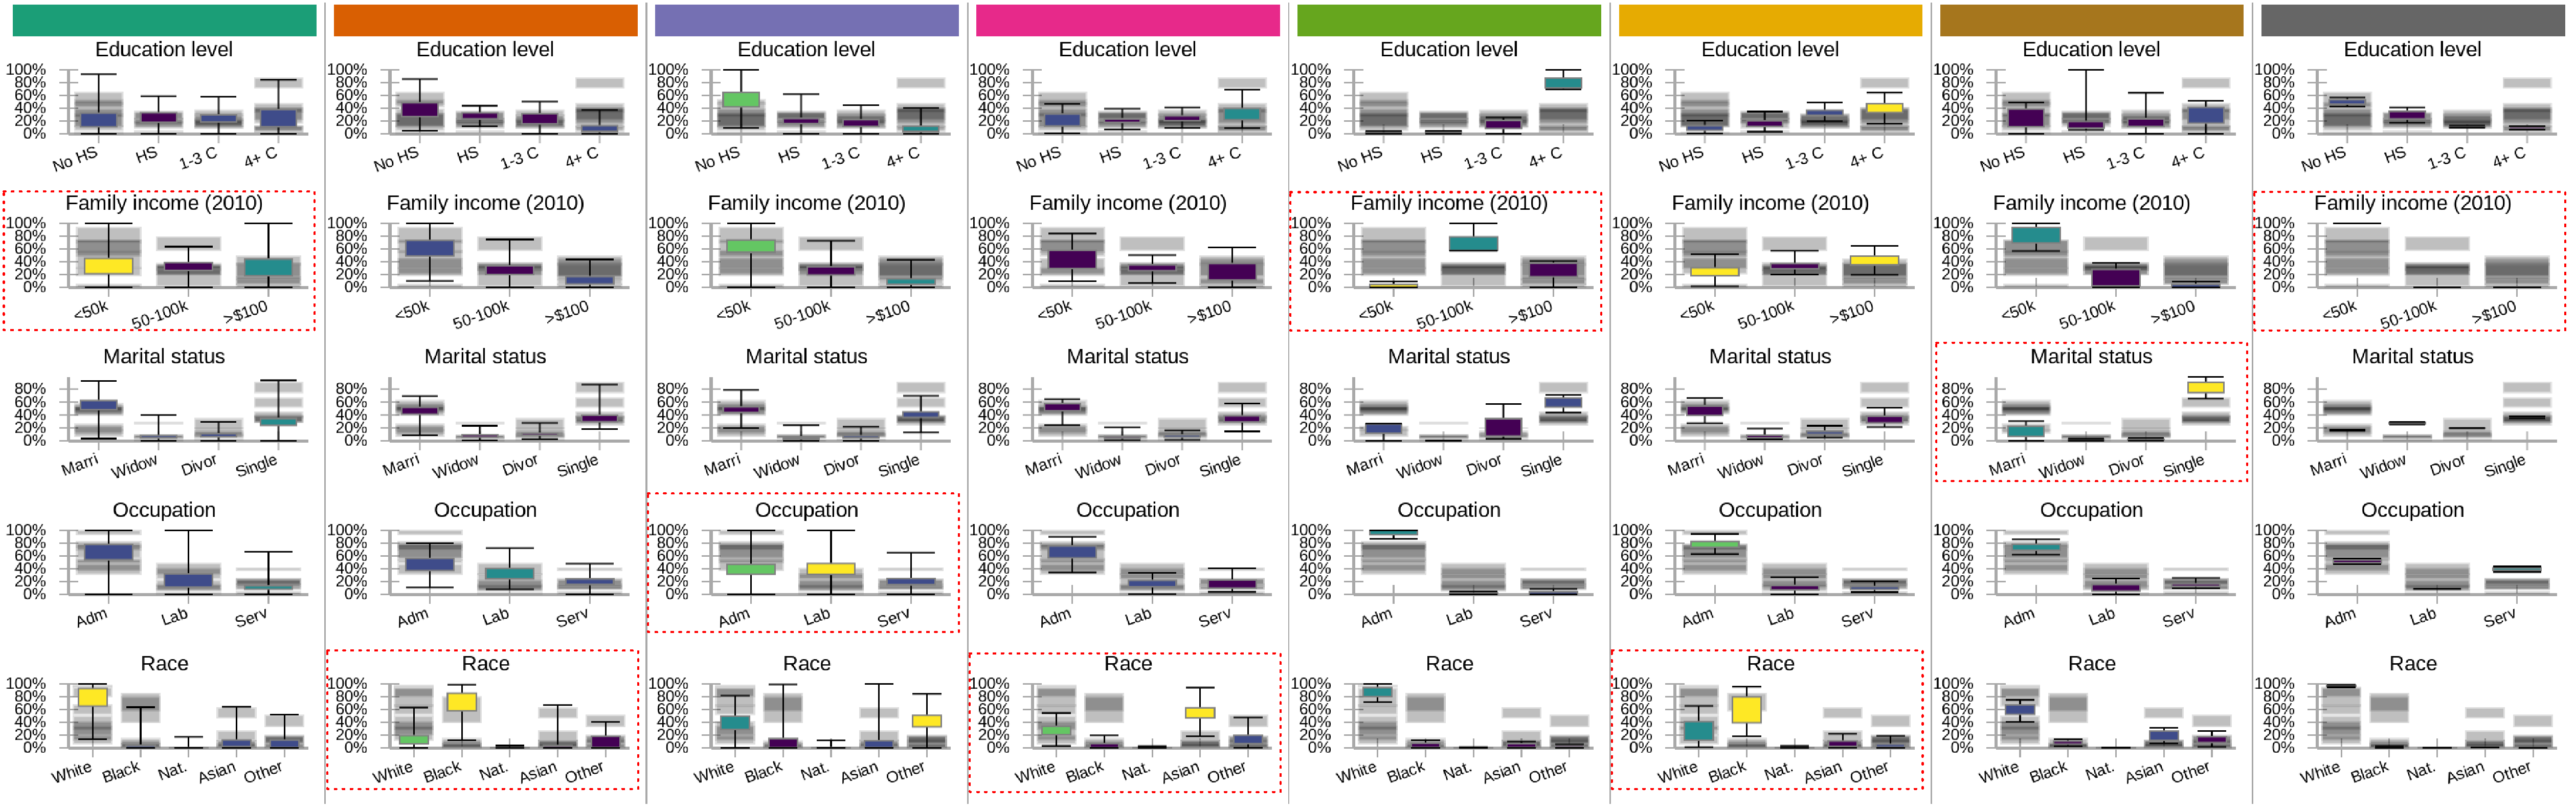
\includegraphics[width=0.95\linewidth]{laAll.pdf}
%     \caption{Full characterisation of the eight clusters found for LA. The red
%      rectangles indicate the most relevant aspects for each
%      cluster.\label{fig:laAll}}
% \end{figure*}

% The  green, orange, and purple clusters present a significant intra-cluster
% variance in most variables, as indicated by extreme whiskers of the boxplots.
% While fifty percent of the CTs in the green cluster have between 20\% and 40\%
% of people in the lowest income bracket, that cluster also includes CTs where
% none and all the population belongs to that bracket. This might indicate that
% this cluster represents different groups of people that are not different enough
% to be separated at this level of the hierarchy. Conversely, the light green,
% brown, and dark grey clusters are different enough to be separated into their
% own clusters at this level, despite being small and ephemeral, including only a
% few CTs. 

% The orange area in the map in Figure~\ref{fig:la} presents movement, indicated by
% the presence of green and purple tones mixed with the orange, which may warrant
% further exploration. By clicking on the orange bar above the boxplot, we select
% all trajectories that contain the orange cluster. The corresponding details are
% illustrated in Figure~\ref{fig:labh}. This shows a location change, where the
% orange cluster is progressively replaced by the purple cluster on its east side,
% and in turn expanding to the west. Interestingly, the population increased, the
% racial profile changed, but the distribution of income was reasonably stable,
% with a higher amount of the population in the lowest income range and very few
% people in the highest income range. Indeed, the income  difference is
% significant when compared to the city-wide distribution.

% \begin{figure}
%     \centering 
%     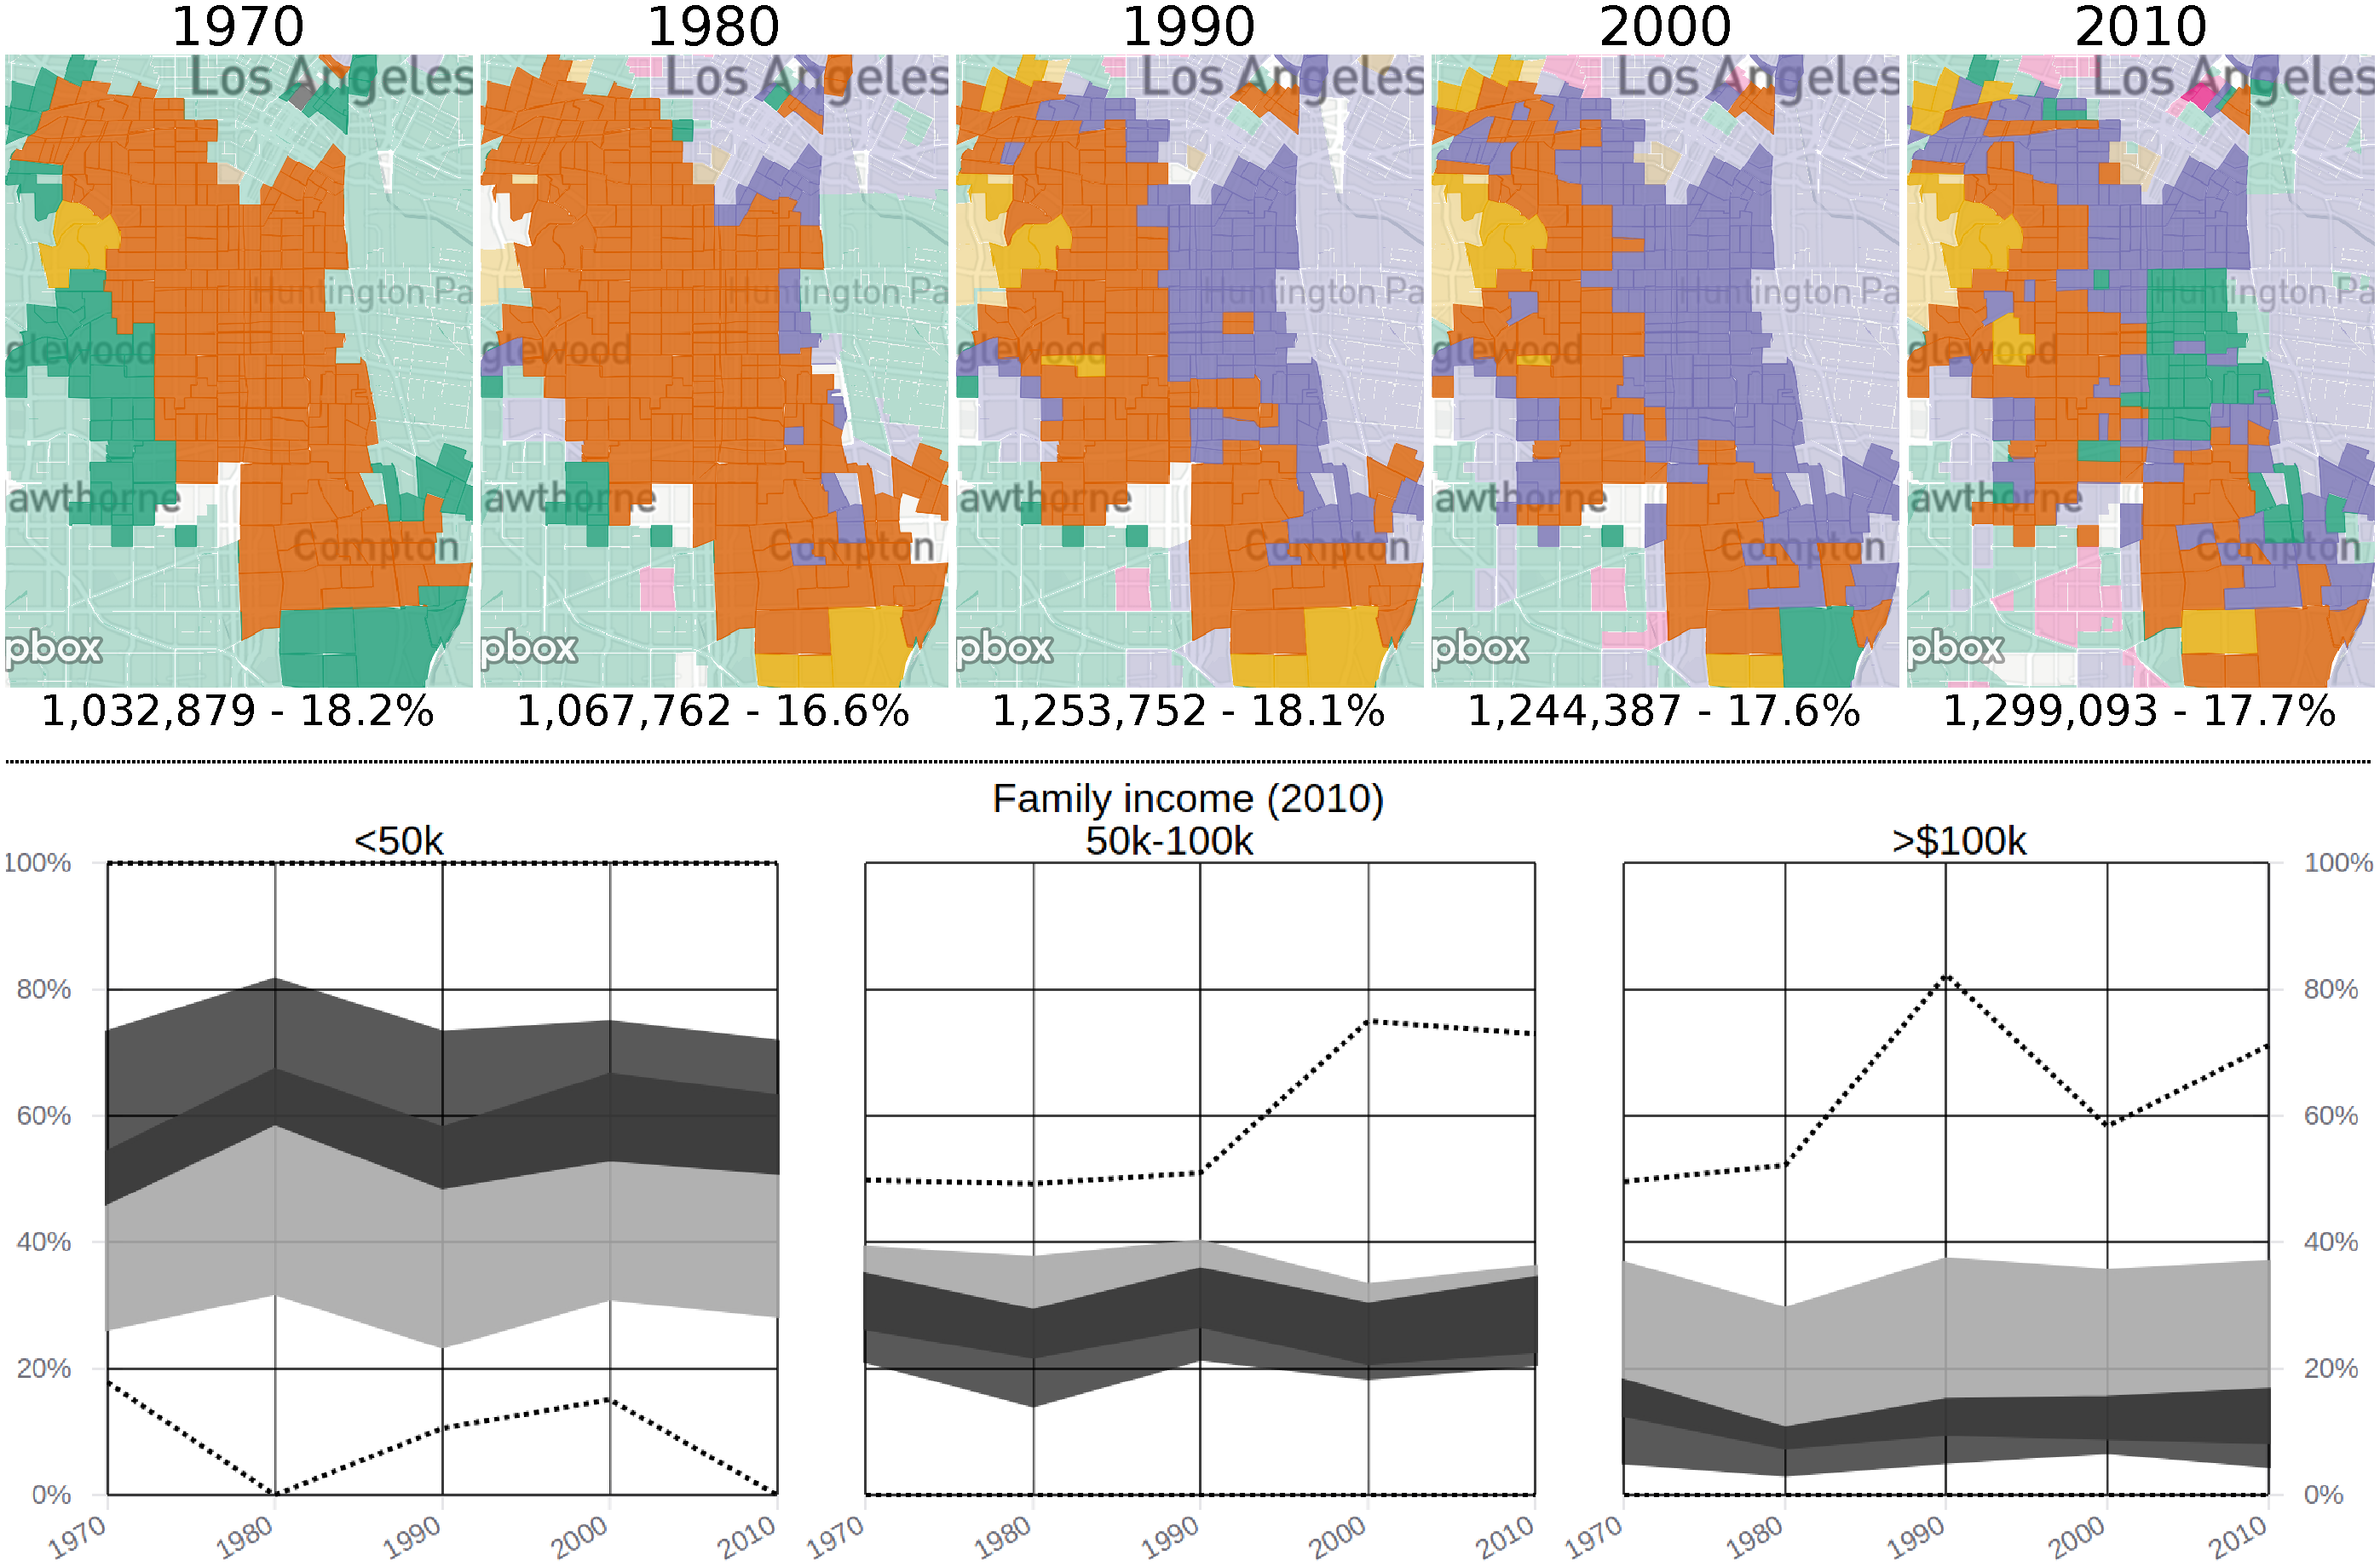
\includegraphics[width=0.75\linewidth]{laBH.pdf}
%     \caption{Top: Geographic changes in the majority Black population cluster
%     (orange) and Labourers cluster (green). Bottom: Income evolution for this
%     region (black) and the whole city (grey).\label{fig:labh}}
% \end{figure}


% A portion of this region is classified into the green cluster in 2010,
% indicating a majority white population. To further understand that change, we
% clear the current selection, and select all regions that changed from orange in
% 1970 to green in 2010, using the transition matrix. A portion of the resulting
% region, near the Florence-Graham region, is depicted in Figure~\ref{fig:laVol},
% along with the temporal evolution of Race. Despite this difference, the other
% aspects are similar to the ones from the region in Figure~\ref{fig:labh}, with
% slightly lower income and education profiles. While the racial aspect changed
% considerably, the economic and educational aspects stayed the same.

% \begin{figure}
%     \centering 
%     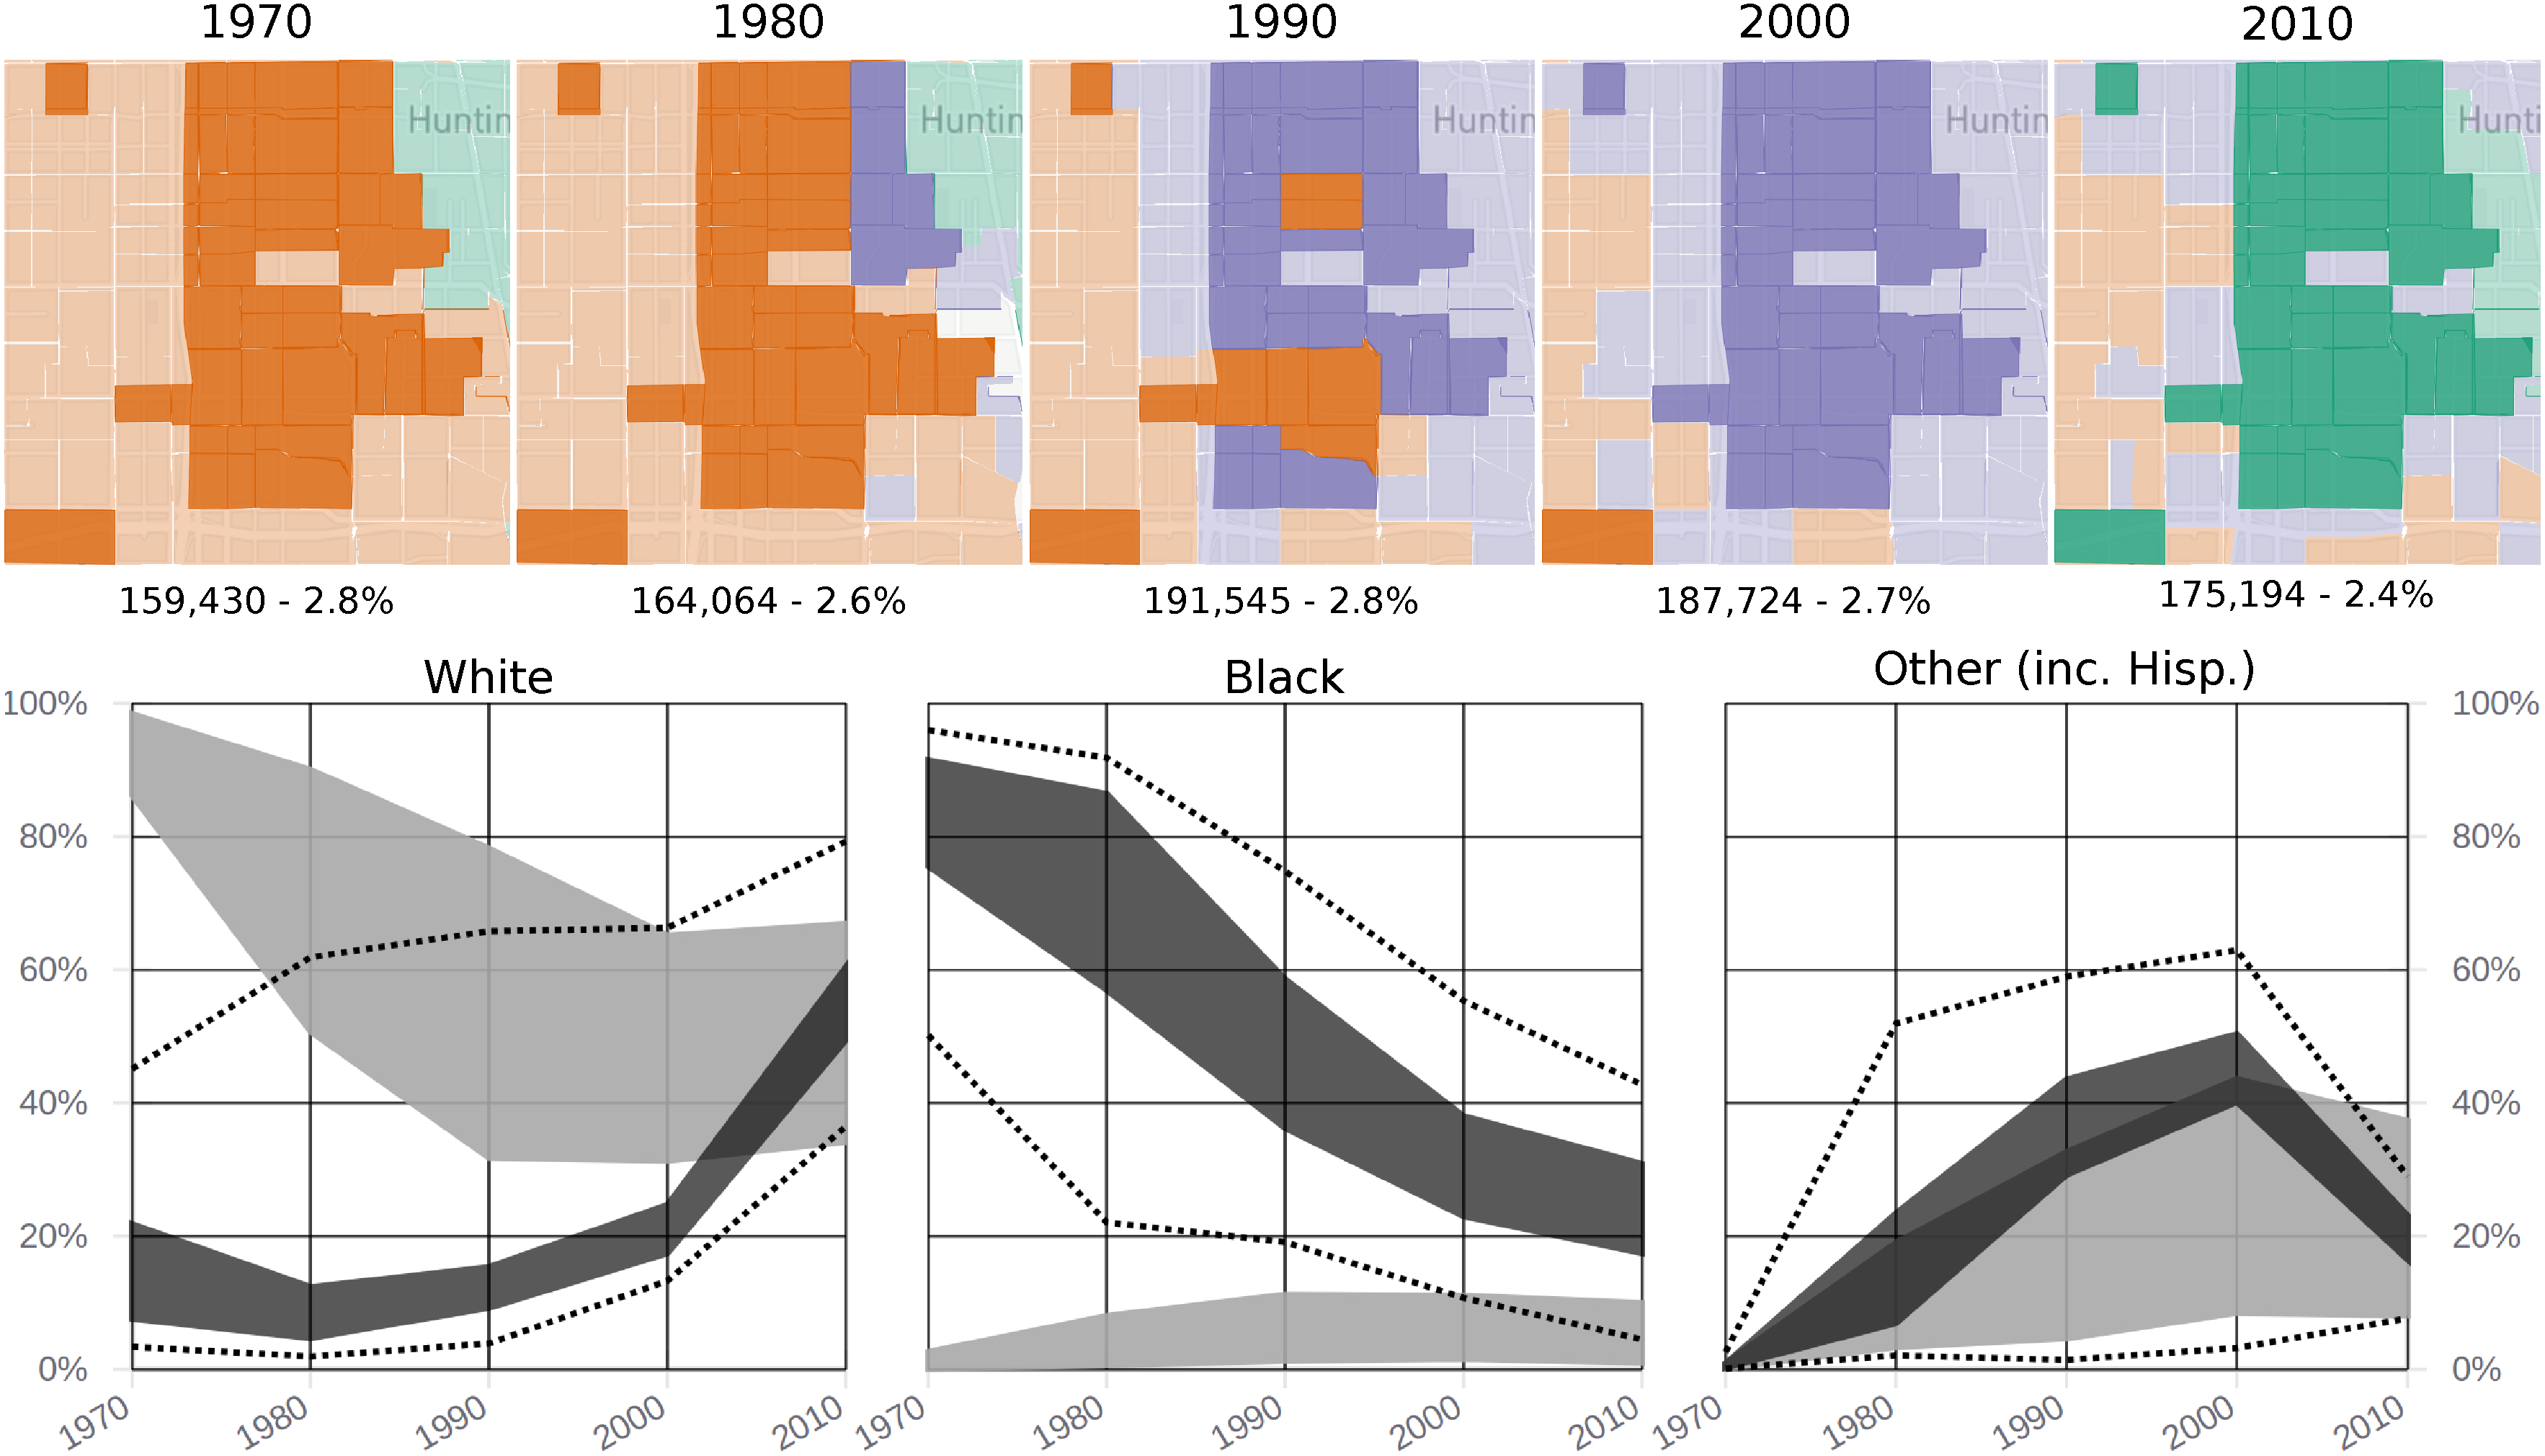
\includegraphics[width=0.75\linewidth]{laVol.pdf}
%     \caption{Details for a volatile region contained in the area of
%          Figure~\ref{fig:labh}. This region went from Black to Hispanic to
%         White.\label{fig:laVol}}
% \end{figure}


% These results are visually similar to the analysis presented by
% Dellmelle~\citep{Delmelle2016}.  What was there identified as 'persistently
% struggling' corresponds to the purple cluster in Figure~\ref{fig:la}; some
% portions of the 'stable elite' cluster, near Inglewood, correspond to the high
% income, high education yellow cluster. The other groups identified by that study
% were clumped by our system into the green cluster, which would be further
% divided if more than eight clusters were to be used. 

% If Toronto illustrates a relatively smooth process of whole-sale
% diversification, Los Angeles shows the ability of our system and method to
% uncover more intensive smaller-scale processes of neighbourhood change. This
% capacity to examine and classify different types of change operating at
% different scales demonstrates the flexibility of the method and tool for
% advancing the more open-ended notion of "neighbourhood" envisioned by recent
% neighbourhood research. 



% \smallskip While Toronto is more dynamic than Los Angeles, possibly due to size
% differences, the volatile regions shown in Figure~\ref{fig:toVol} did not change
% as quickly or dramatically as the ones shown in Figure~\ref{fig:laVol}, which
% involved twice as many people. We found this trend to be related to the
% countries themselves, Canadian cities have larger areas undergoing slow, gradual
% changes, whereas American cities have more general stability, but quicker
% changes in smaller scales. The supplementary material contains brief summaries
% of all the regions accessible in this prototype.





\section{Expert feedback}
\label{sec:expert}
As our method and tool are novel to the field, and somewhat exotic,  we
subjected them to the critical scrutiny of experts. We contacted academic and
industry experts in sociology and urban sciences to solicit their evaluation of
our methodology. They had access to the prototype tool, a descriptive
documentation of the features (included in the supplementary material), and a
sequence of documentation videos illustrating how to perform specific tasks. The
documentation explains which datasets are used and how the data is represented
and processed, noting explicitly that there is no geographic harmonisation. We
focused our inquires on the results obtained, asking if they found anything
interesting in the data. The message sent and their full response is included in
the supplementary material. Each of the five experts is identified by a letter,
from A to E. 



The overall overall response of the experts was positive,  mentioning that the
prototype allows them to analyse census data without the additional work of
obtaining and cleaning the data (A, B, E), and it allows the inclusion of
geographic visual analysis tools in their research process (D). It enables the
users to tell different stories about neighbourhoods/cities and their changes
(A), visualise the relationship between key urban variables over time (D),
offering a quick way to identify particular neighbourhoods that one may be
interested in studying more in depth around a particular issue or efficiently
understanding the context of an area (E).  Indeed, the experts identified
gentrification processes in Manhattan (B) and Dallas (E), reinforced a
hypothesis for occupational clustering (D), and highlighted how the method can
be used to compare neighbourhoods and cities (A). In summary, their view was that
the proposed methodology can be a viable alternative for the visual analytics of
evolving demographic data.



The interface was "easy to navigate" (B), but it was also considered
"overwhelming" (A), "intimidating" (E), and "tricky to interpret" (C), possible
side-effects of our effort to increase  representational accuracy, where we
avoided using simplified representation or labels. Identifying clusters by their
most relevant variables was welcome, but the overlap of information from
different clusters in the boxplot was "a bit confusing" (C) when colour was not
present. Further, most clusters can be sufficiently characterised using only the
most relevant aspect, but this is not generally true. 


While the map of trajectories was mentioned as a "good summary map", how it
related to the clustering method was unclear (C). The methods include different
options on how the colours are used, but both are works in progress since reliably
representing several distinct entities using colours is humanly unfeasible.
Indeed, the number of distinguishable colours was a significant constraint, we
found indications that more clusters should be used in some cases, even if eight
clusters is more than what is traditionally considered in these analyses.
Conversely, increasing the number of clusters would also complicate the
interpretation of the results.


The experts also mentioned the poor responsiveness of the method when changes in
the clustering parameters required server-side processing (B,D). Indeed, the
current implementation can take a few minutes to cluster regions with high
number of CTs, like Los Angeles or Brooklyn. Server-processing reduced the
amount of data transferred to client, but it might increase the response time
under load. We implemented a caching policy that greatly improved the
performance, but fully pre-processing the results is not practical due to size
of the parameter space.

Most of the experts demonstrated interest in using our method in their research
(A, B, D, E), aiming to use the census data as a backdrop for other datasets,
providing demographic context. They also mentioned the need to export subsets of
data, plots, and maps to be used in reports and publications (C, D, E). More
importantly, while these experts were aware that our method does not perform
geographic harmonisation, none of them mention it. We did not specifically ask
if this difference led to unexpected results, but rather if they found
interesting insights. 